\documentclass[a4paper,12pt]{article}

\usepackage{other/lab_preamble}

\numberwithin{equation}{section}

\begin{document}

\LabTitle{1.4.8}{Измерение модуля Юнга методом акустического резонанса}

\tableofcontents

\listoffigures

\listoftables

\newpage

\textbf{Цель работы}:
\begin{enumerate}
  \item исследовать явление акустического резонанса в тонком стержне.
  \item измерить скорость распространения продольных звуковых колебаний в тонких стержнях из различных материалов и различных размеров.
  \item измерить модули Юнга различных материалов.
\end{enumerate}

\textbf{Приборы}:
\begin{enumerate}
  \item генератор звуковых частот
  \item частотомер
  \item осциллограф
  \item электромагнитные излучатель и приёмник колебаний
  \item набор стержней из различных материалов
\end{enumerate}

\section{Краткая Теория.}
\subsection{Введение.}
Закон гука:
\begin{equation}
  \sigma =  \varepsilon E
  \label{eq:1}
\end{equation}

Малые деформации твердых тел вызывают волны, которые называют акустическими или звуковыми.
Волны сжатия/растяжения, распространяющиеся вдоль оси, по которой происходит деформация, называются продольными.

\begin{equation}
  u =  \sqrt{\frac{E}{\rho}}
  \label{eq:2}
\end{equation}
, где u - скорость распространения продольной акустической волны, 
$\rho$ - плотность среды.

Характерные значения модуля Юнга металлов лежат в диапазоне $E \sim (10^{10} - 10^{12}) \text{Па}$, так как при плотности $\rho \sim 10^4 \text{кг}/\text{м}^3$ характерные значения скорости звука в
твёрдых телах составляют $u \sim (10^3 - 10^4) \text{м/с}$.

Рассмотрим стержень постоянного круглого сечения, радиус R которого много меньше его длины L. С точки зрения распространения волн стержень можно считать тонким, если длина $\lambda$ звуковых волн в нём велика по сравнению с его радиусом: $\lambda \gg R$.

\subsection{Уравнение волны в тонком стержне}
Пусть плоскость среды, находящаяся исходно в точке x,
сместилась к моменту t на расстояние $\xi(x,t)$.

\begin{equation}
  \varepsilon = \partderiv{\xi}{x}
  \label{eq:3}
\end{equation}

\eqref{eq:1} implies

\begin{equation}
  \sigma =  \varepsilon E = E \partderiv{\xi}{x}
  \label{eq:4}
\end{equation}

\begin{figure} [H] \center
  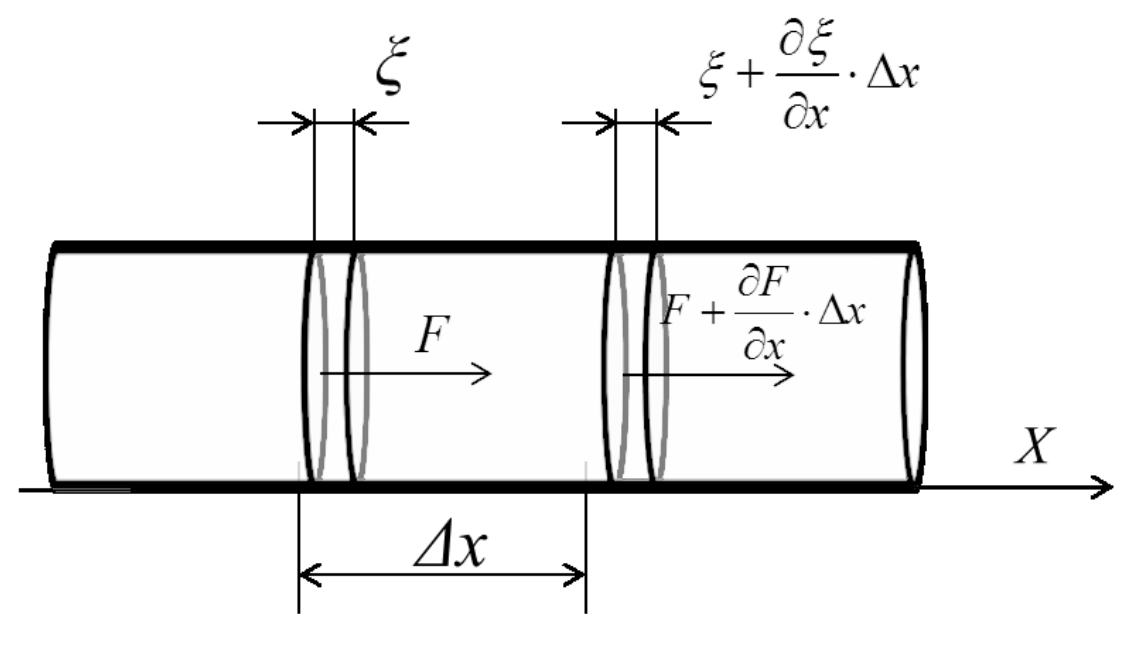
\includegraphics[scale=0.3]{data/pic1.png}
  \caption{Силы, действующие на элемент стержня при продольных колебаниях}
  \label{pic:1}
\end{figure}

\begin{equation}
  \Delta F = S \D{x} \partderiv{\sigma}{x} = 
  \partderiv[2]{\xi}{x} E S \D{x}
  \label{eq:5}
\end{equation}

Волновое уравнение:
\begin{equation}
  \partderiv[2]{\xi}{t} = u^2 \partderiv[2]{\xi}{x}
  \label{eq:6}
\end{equation}

При $\lambda \ll R$:
\[ u_i = \sqrt{\frac{E}{\rho} \cdot \frac{1-\mu}{(1+\mu)(1-2\mu)}} \]
\label{eq:ui}

\subsection{Бегущие акустические волны. Скорость волны}
Общее решение волнового ур-ия \eqref{eq:6}:
\begin{equation}
  \xi(x,t) = \phi_1(x-ut) + \phi_2(x+ut)
  \label{eq:7}
\end{equation}

\subsection{Собственные колебания стержня. Стоячие волны}
В случае гармонического возбуждения:
\begin{equation}
  \xi(x,t) = A_1 \sin{(\omega t - kx + \varphi_1)} + 
  A_2 \sin{(\omega t + kx + \varphi_2)}
  \label{eq:8}
\end{equation}
$\omega = 2\pi f$ - циклическая частота, 
$k = \frac{2\pi}{\lambda}$ - волновое число или пространственная частота волны.

Если конци не закреплены:
\begin{equation}
  \sigma(0) = 0 \implies \partderiv{\xi}{x} (x = 0) = 0,\ (1)
  \sigma(L) = 0 \implies \partderiv{\xi}{x} (x = L) = 0\ (2) 
  \label{eq:9}
\end{equation}

\eqref{eq:8} и \eqref{eq:9} $\implies$
\begin{equation}
  A_1 = A_2 \label{eq:10}
\end{equation}
\begin{equation}
  \varphi_1 = \varphi_2 \label{eq:11}
\end{equation}

$\eqref{eq:8}, \eqref{eq:10}, \eqref{eq:11} \implies$
\begin{equation}
  \xi(x,t) = 2A \cdot \cos{kx} \cdot \sin{(\omega t \varphi)}
  \label{eq:12}
\end{equation}
Колебания вида \eqref{eq:12} называют гармоническими стоячими волнами.

Воспользуемся вторым граничным условием \eqref{eq:9}:

Воспользуемся вторым граничным условием \eqref{eq:9} применительно к функции \eqref{eq:12}. В результате придём к уравнению $\sin(kL) = 0$, решения которого определяют набор допустимых значений волновых чисел $k$:

\begin{equation}
  k_n L = \pi n, \quad n \in \N
  \label{eq:13}
\end{equation}

выражая \eqref{eq:13} через длину волны $\lambda = \frac{2 \pi}{k},$, получим

\begin{equation}
  \lambda_n = \frac{2L}{n}, \quad n \in \N
  \label{eq:14}
\end{equation}
Таким образом, для возбуждения стоячей волны на длине стержня должно укладываться целое число полуволн.

Допустимые значения частот:
\begin{equation}
  f_n = \frac{u}{\lambda_n} = n \frac{u}{2L}, \quad n \in \mathbb{N}
  \label{eq:15}
\end{equation}
называют собственными частотами колебаний стержня длиной $L$. Именно при совпадении внешней частоты с одной из частот $f_n$ в стержне возникает акустический резонанс.
        
Зависимость амплитуды смещения от координаты для собственных колебаний стержня с незакреплёнными концами при $n = 1,2,3$ представлена на рис. \ref{pic:2}.

\begin{figure} [H] \center
  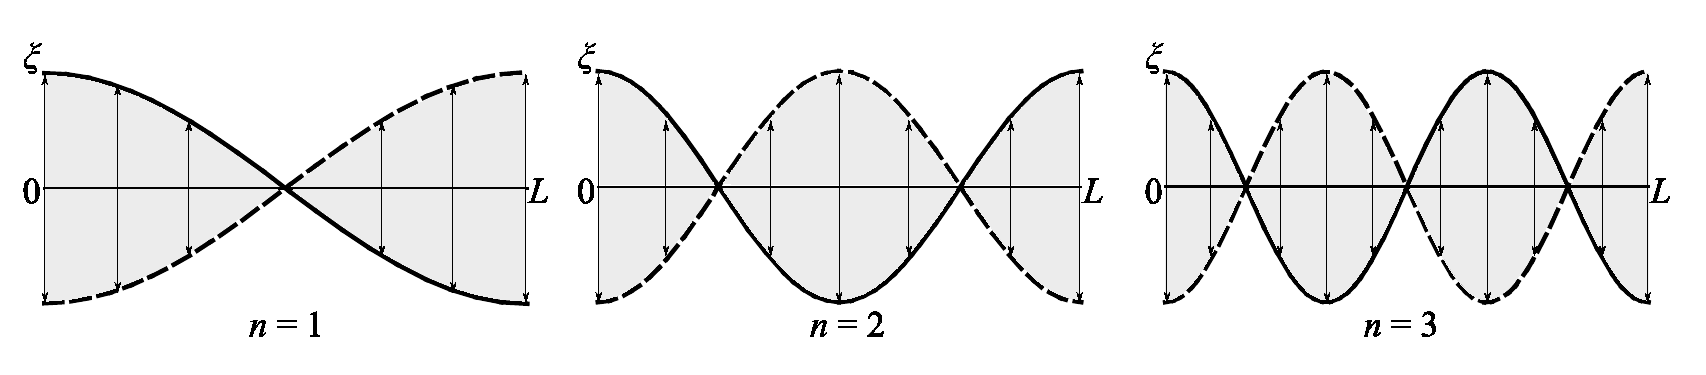
\includegraphics[scale=0.4]{data/pic2.png}
  \caption[Гармоники]{Собственные продольные колебания стержня с незакреплёнными концами}
  \label{pic:2}
\end{figure}

\subsection{Схема.}

\begin{figure} [H] \center
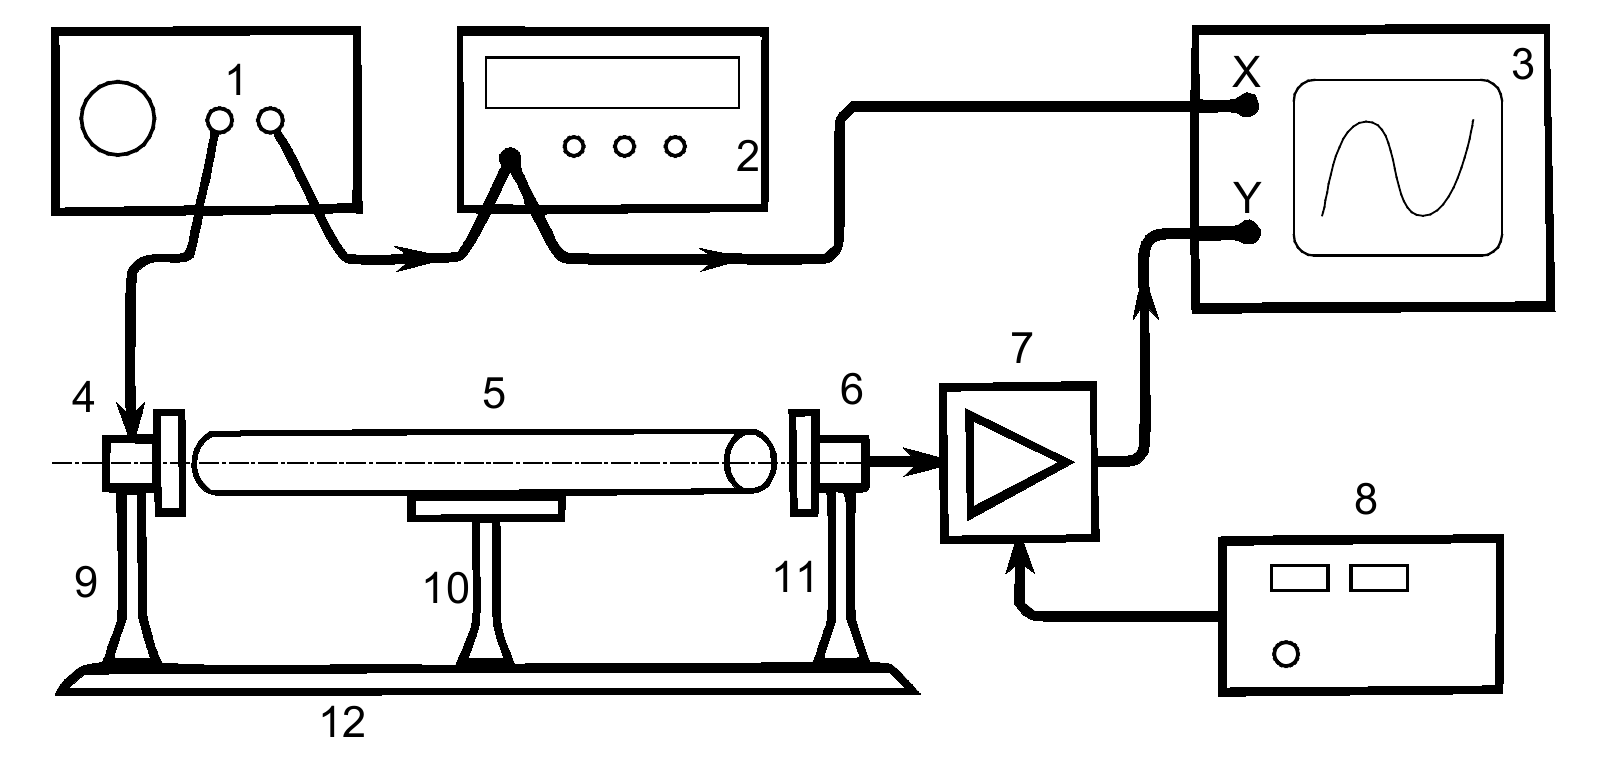
\includegraphics[scale=0.4]{data/pic3.png}
\caption{Схема установки.}
\begin{description}
  \item[1] - генератор звуковой частоты
  \item[2] - частотомер
  \item[3] - осциллограф
  \item[4] - электромагнит-возбудитель
  \item[5] - образец
  \item[6] - электромагнитный приемник
  \item[7] - усилитель звуковой частоты
  \item[8] - блок питания усилителя
  \item[9 и 11] - стойки крепления электромагнитов
  \item[10] - стойка крепления образца
  \item[12] - направляющая
\end{description}
\label{pic:3}
\end{figure}

\begin{figure} [H] \center
  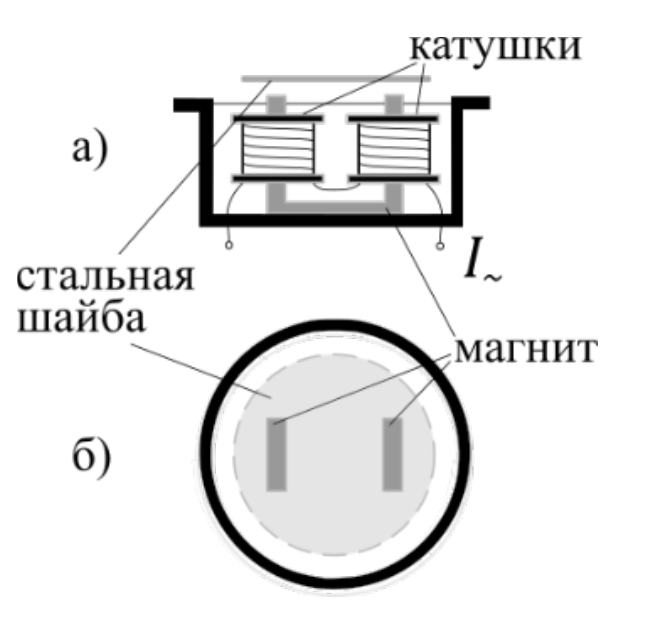
\includegraphics[scale=0.4]{data/pic4.png}
  \caption[Электромагнитный датчик]{Электромагнитный датчик: а) вид спереди, б) вид сверху}
  \label{pic:4}
\end{figure}

\section{Выполнение.} \label{Выполнение}
\begin{enumerate}
\item \label{Выполнение:1}
  Познакомимся с основными органами управления электронного осциллографа. По техническому описанию к работе проведем предварительную настройку осциллографа и звукового генератора.
\item \label{Выполнение:2}
  Раздвиним датчики и поместим на подставку между ними исследуемый стержень. Рекомендуется использовать сначала медный стержень, потом железный и дюралюминивый. Длина стержней известна.
  \[ L = (60.0 \pm 0.1)\ \cm \]

\item \label{Выполнение:3}
  Разместим электромагниты напротив торцов стержня как можно ближе, но так, чтобы они не соприкасались.

\item \label{Выполнение:4}
Предварительно определим диапазон частот генератора, в котором целесообразно искать резонансы. Для этого оценим частоту первого резонанса по формуле перестраивая $f_1 = \frac{u}{2L}$, воспользовавшись табличным значением скорости. (см. таблицу \ref{table:1})

% Таблица со сокоростями волн и предполагаемыми частотами первого резонанса  в стержнях
\begin{table} [H] \center
\begin{tabular}{l|ll}
&u, м/с&$f_1$, кГц\\
\hline
Медь&3790&3.16\\
Железо&5170&4.31\\
дюралюминий&5150&4.29\\
\end{tabular}
\caption{Таблица со сокоростями волн и предполагаемыми частотами первого резонанса  в стержнях. \label{table:1}}
\end{table}


\item \label{Выполнение:5}
\quad Вблизи расчетной частоты $f_1$ найдем резонанс. В резонансе амплитуда волн максимальна, чтобы достичь максимальной амплитуды, мы можем делать три вещи: менять частоту генератора, менять положение электромагнитов и настраивать осциллограф. \par
\quad Измерять амплитуду на осциллографе мы можем в двух режимах: фигурой Лиссажу и синусоидой. В первом случае на экране будет элипс, который резко увеличится в размерах или даже превратиться в \qts{бочку}, при достижении резонанса. Во втором случае, амплитуда синусоиды резко увеличится, при достижении резонанса.

\item \label{Выполнение:6}
  Определим значение первой резонансной частоты $f_1$ по частотометру. (см. таблицу \ref{table:2})

\item \label{Выполнение:7}
  Получим резонансы на частотах, соответствующих следующим
(кратным) гармоникам. Для этого, плавно перестраивая генератор, добьемся резонанса вблизи частот $f_n \approx nf_1$. Найдите как можно больше гармоник, мы нашли 7. (см. таблицу \ref{table:2}). \par
\textbf{Замечание.}
\quad Не учитывая человеческий фактор, погрешность измерения f равна последнему разряду на частотометре, т.е. $10^{-6} \kHz$, однако, в действительности, погрешность значительно больше, так как настроить генератор на частоту с такой точностью просто невозможно, при этом, даже если вы настроились на правильною частоту, не факт, что вы сможете распознать ее как резонансную. \par
\quad По моим ощущениям, погрешность составляет 10-50 Гц. \par
\quad Даже так, если быть неаккураным, то могут получиться сильные отконения от ожидаемых значений, как получилось у нас с червертой и пятой гармоникой меди (см. рис. \ref{pic:6}).


% Частотометр
\begin{figure} [H] \center
  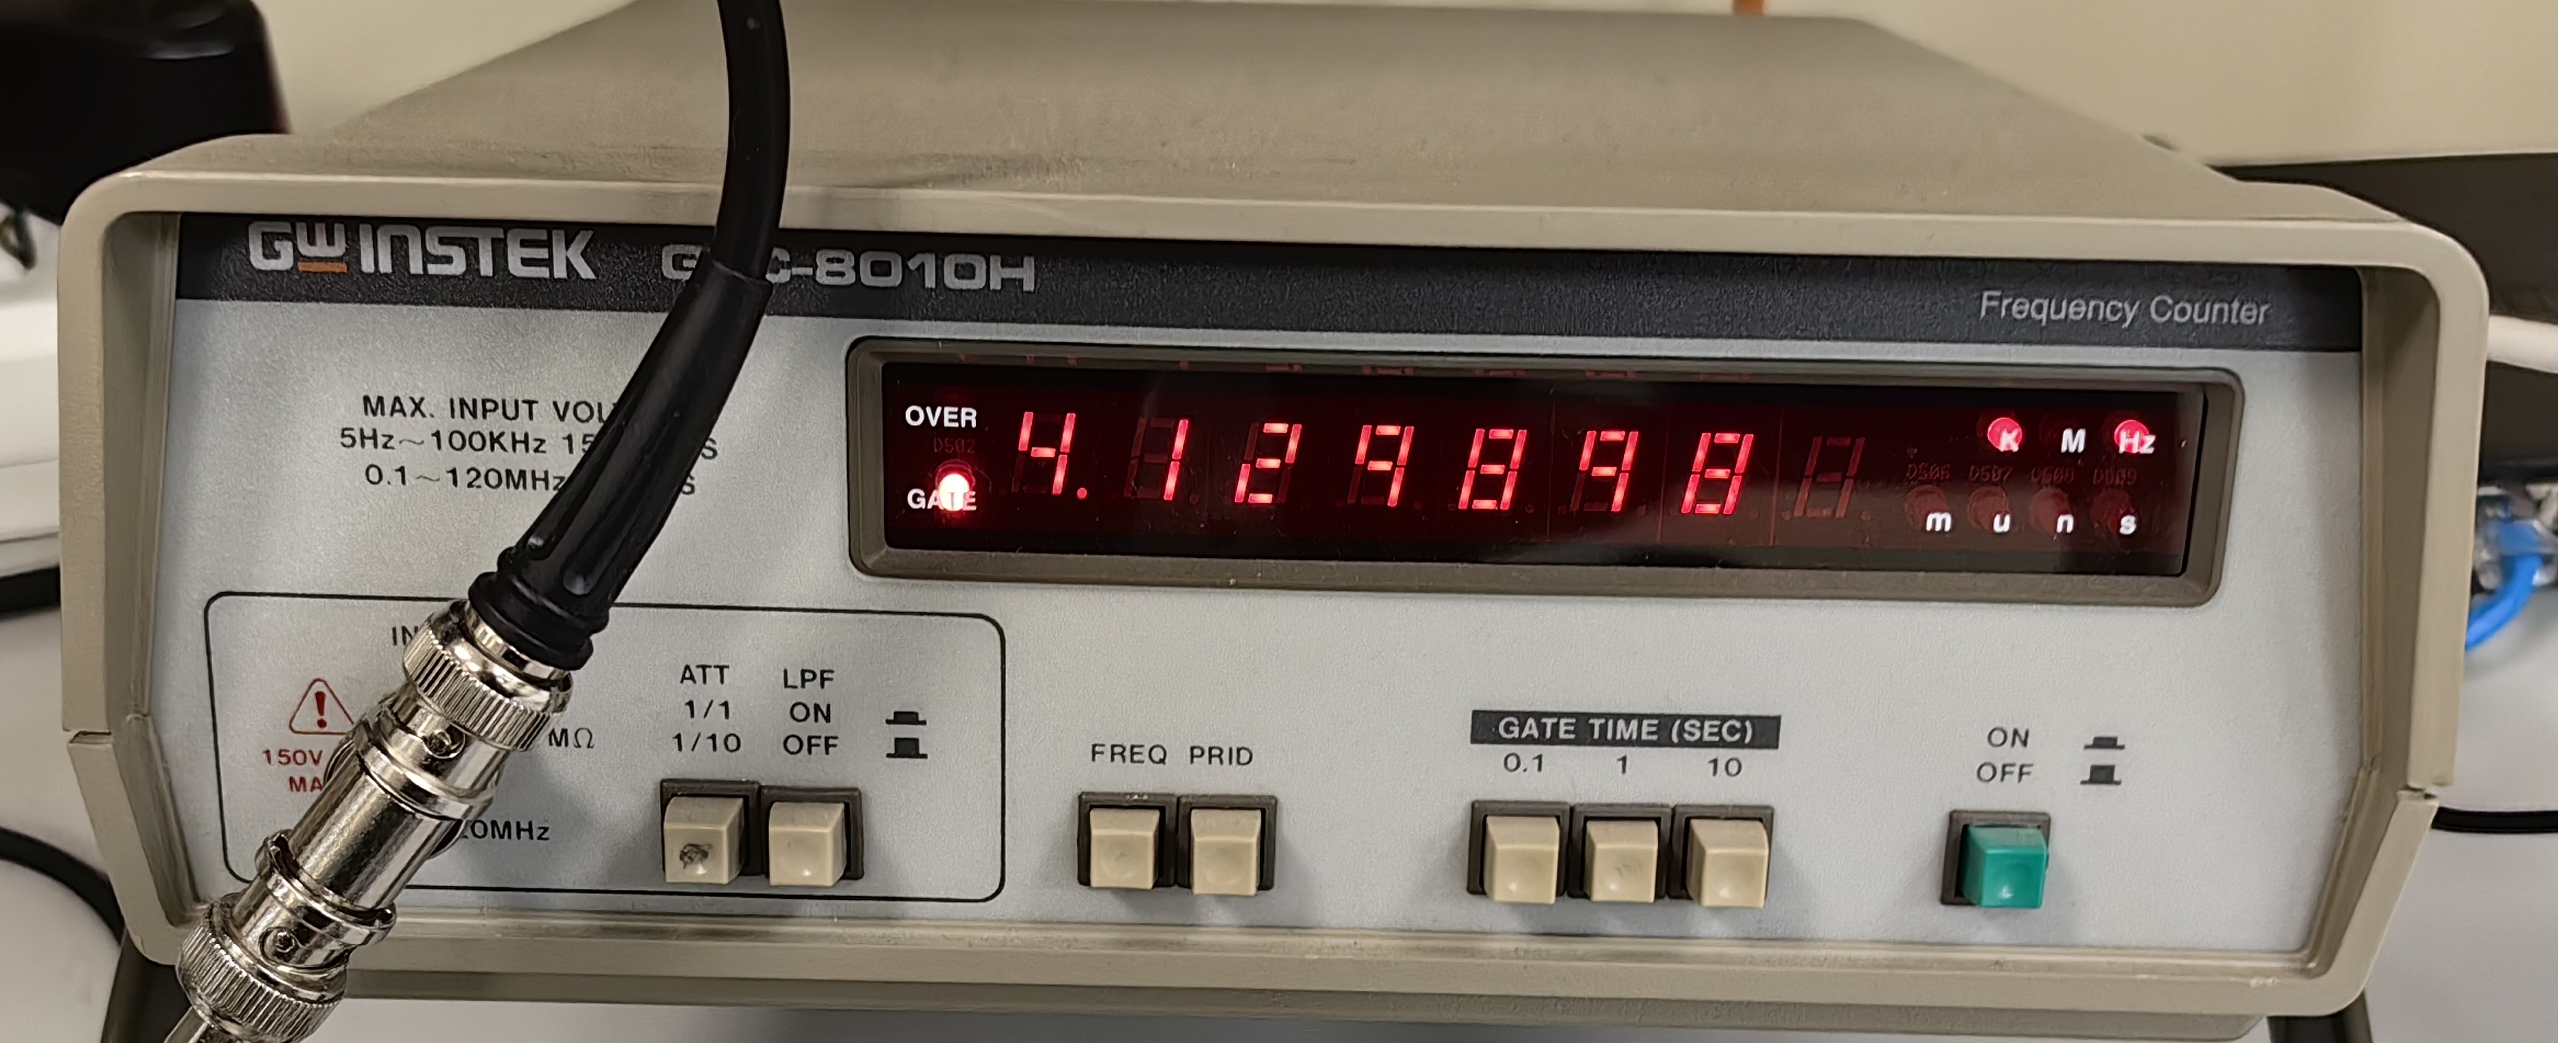
\includegraphics[scale=0.15]{data/частотометр(2)}
  \caption{Частотометр.} 
  \label{pic:Hz meter}
\end{figure}

% Таблица с гармониками
\begin{table} [H] \center
\resizebox{\columnwidth}{!}{
\begin{tabular}{l|lll|lll|lll}
&Медь&&&Железо&&&Дюраль&&\\
\hline
&f, кГц&$\sigma_f$, кГц&$\eps_f$&f, кГц&$\sigma_f$, кГц&$\eps_f$&f, кГц&$\sigma_f$, кГц&$\eps_f$\\
\hline
$f_1$&\ 3.25&0.01&0.31\%&\ 4.13&0.01&0.24\%&\ 4.25&0.01&0.23\%\\
$f_2$&\ 6.49&0.01&0.15\%&\ 8.27&0.01&0.12\%&\ 8.50&0.01&0.12\%\\
$f_3$&\ 9.72&0.01&0.10\%& 12.40&0.01&0.08\%& 12.78&0.01&0.08\%\\
$f_4$& 12.26&0.01&0.08\%& 16.55&0.01&0.06\%& 17.02&0.01&0.06\%\\
$f_5$& 16.50&0.01&0.06\%& 20.68&0.01&0.05\%& 21.30&0.01&0.05\%\\
$f_6$& 19.48&0.01&0.05\%& 24.81&0.01&0.04\%& 25.38&0.01&0.04\%\\
$f_7$& 22.72&0.01&0.04\%& 28.94&0.01&0.03\%& 30.22&0.01&0.03\%\\
\end{tabular}
}
\caption{Гармоники.}
\label{table:2}
\end{table}

\item \label{Выполнение:8}
  Найдем плотность стержня, для этого измерим массу, диаметр и длину восьми маленьких экземпляров из исследуемого материала. (см. таблицу \ref{table:3} и \ref{table:4})

% Таблица с измерениями маленьких экземпляров стержней
\begin{table} [H] \center
\begin{tabular}{ll|lll|lll|lll}
&&m, г&$\sigma_m$, г&$\eps_m$&d, см&$\sigma_d$, см&$\eps_d$&l, см&$\sigma_l$, см&$\eps_l$\\
\hline
Медь
&1&29.110&0.001&0.003\%&1.19&0.01&0.84\%&2.98&0.01&0.34\%\\
&2&30.110&0.001&0.003\%&1.20&0.01&0.83\%&3.10&0.01&0.32\%\\
&3&9.461&0.001&0.003\%&1.18&0.01&0.85\%&3.00&0.01&0.33\%\\
&4&39.385&0.001&0.003\%&1.20&0.01&0.83\%&3.98&0.01&0.25\%\\
&5&40.990&0.001&0.002\%&1.20&0.01&0.83\%&4.00&0.01&0.25\%\\
&6&40.352&0.001&0.002\%&1.20&0.01&0.83\%&4.05&0.01&0.25\%\\
&7&38.714&0.001&0.003\%&1.18&0.01&0.85\%&4.02&0.01&0.25\%\\
&8&41.334&0.001&0.002\%&1.20&0.01&0.83\%&4.14&0.01&0.24\%\\
\hline
Железо
&1&28.107&0.001&0.004\%&1.23&0.01&0.81\%&3.12&0.01&0.32\%\\
&2&26.159&0.001&0.004\%&1.21&0.01&0.83\%&2.99&0.01&0.33\%\\
&3&26.029&0.001&0.004\%&1.20&0.01&0.83\%&2.96&0.01&0.34\%\\
&4&35.185&0.001&0.003\%&1.20&0.01&0.83\%&4.00&0.01&0.25\%\\
&5&34.941&0.001&0.003\%&1.20&0.01&0.83\%&3.96&0.01&0.25\%\\
&6&35.137&0.001&0.003\%&1.20&0.01&0.83\%&4.00&0.01&0.25\%\\
&7&36.923&0.001&0.003\%&1.19&0.01&0.84\%&4.11&0.01&0.24\%\\
&8&37.088&0.001&0.003\%&1.20&0.01&0.83\%&4.12&0.01&0.24\%\\
\hline
Дюраль
&1&\ 9.490&0.001&0.011\%&1.22&0.01&0.82\%&3.10&0.01&0.32\%\\
&2&\ 9.195&0.001&0.011\%&1.19&0.01&0.84\%&3.10&0.01&0.32\%\\
&3&\ 8.990&0.001&0.011\%&1.20&0.01&0.83\%&3.00&0.01&0.33\%\\
&4&\ 9.260&0.001&0.011\%&1.19&0.01&0.84\%&3.08&0.01&0.32\%\\
&5&12.187&0.001&0.008\%&1.19&0.01&0.84\%&4.00&0.01&0.25\%\\
&6&12.461&0.001&0.008\%&1.18&0.01&0.85\%&4.14&0.01&0.24\%\\
&7&12.487&0.001&0.008\%&1.18&0.01&0.85\%&4.15&0.01&0.24\%\\
&8&13.228&0.001&0.008\%&1.24&0.01&0.81\%&4.13&0.01&0.24\%\\
\end{tabular}
\caption{Измерения характеристик маленьких экземпляров стержней}
\label{table:3}
\end{table}

% Таблица с плотностями стержней
\begin{table} [H] \center
\begin{tabular}{l|lll}
&$\rho, \gr/\cm^3$&$\sigma_\rho, \gr/\cm^3$&$\eps_\rho$\\
\hline
Медь&8.83&0.21&2.4\%\\
Железо&7.79&0.21&2.7\%\\
дюралюминий&2.69&0.07&2.6\%\\
\end{tabular}
\caption{Плотность стержней.}
\label{table:4}
\end{table}


\item \label{Выполнение:9}
  Определим среднее значение диаметра исследуемого стержня, проверим, что стержень\\ действительно \qts{тонкий}, т.е. $R/\lambda \ll 1$.

  \[ d = (1.20 \pm 0.02)\ \cm, \quad \eps_d = 1.5\%\]

\item \label{Выполнение:10}
  Проведем опыты 2-9 для каждого стержня (см. таблицу \ref{table:2})

\item[11*.] \label{Выполнение:11}
\quad Для одного из стержней проведем дополнительный опыт: при половинной частоте $f = f_1 / 2$ добьемся на экране осциллографа фигуры Лиссажу в режиме "X-Y". (см. рис. \ref{pic:6}) \par
\quad Как объяснить это явлениеe, я не догадался.

% Картинка с бабочкой
\begin{figure} [H] \center
  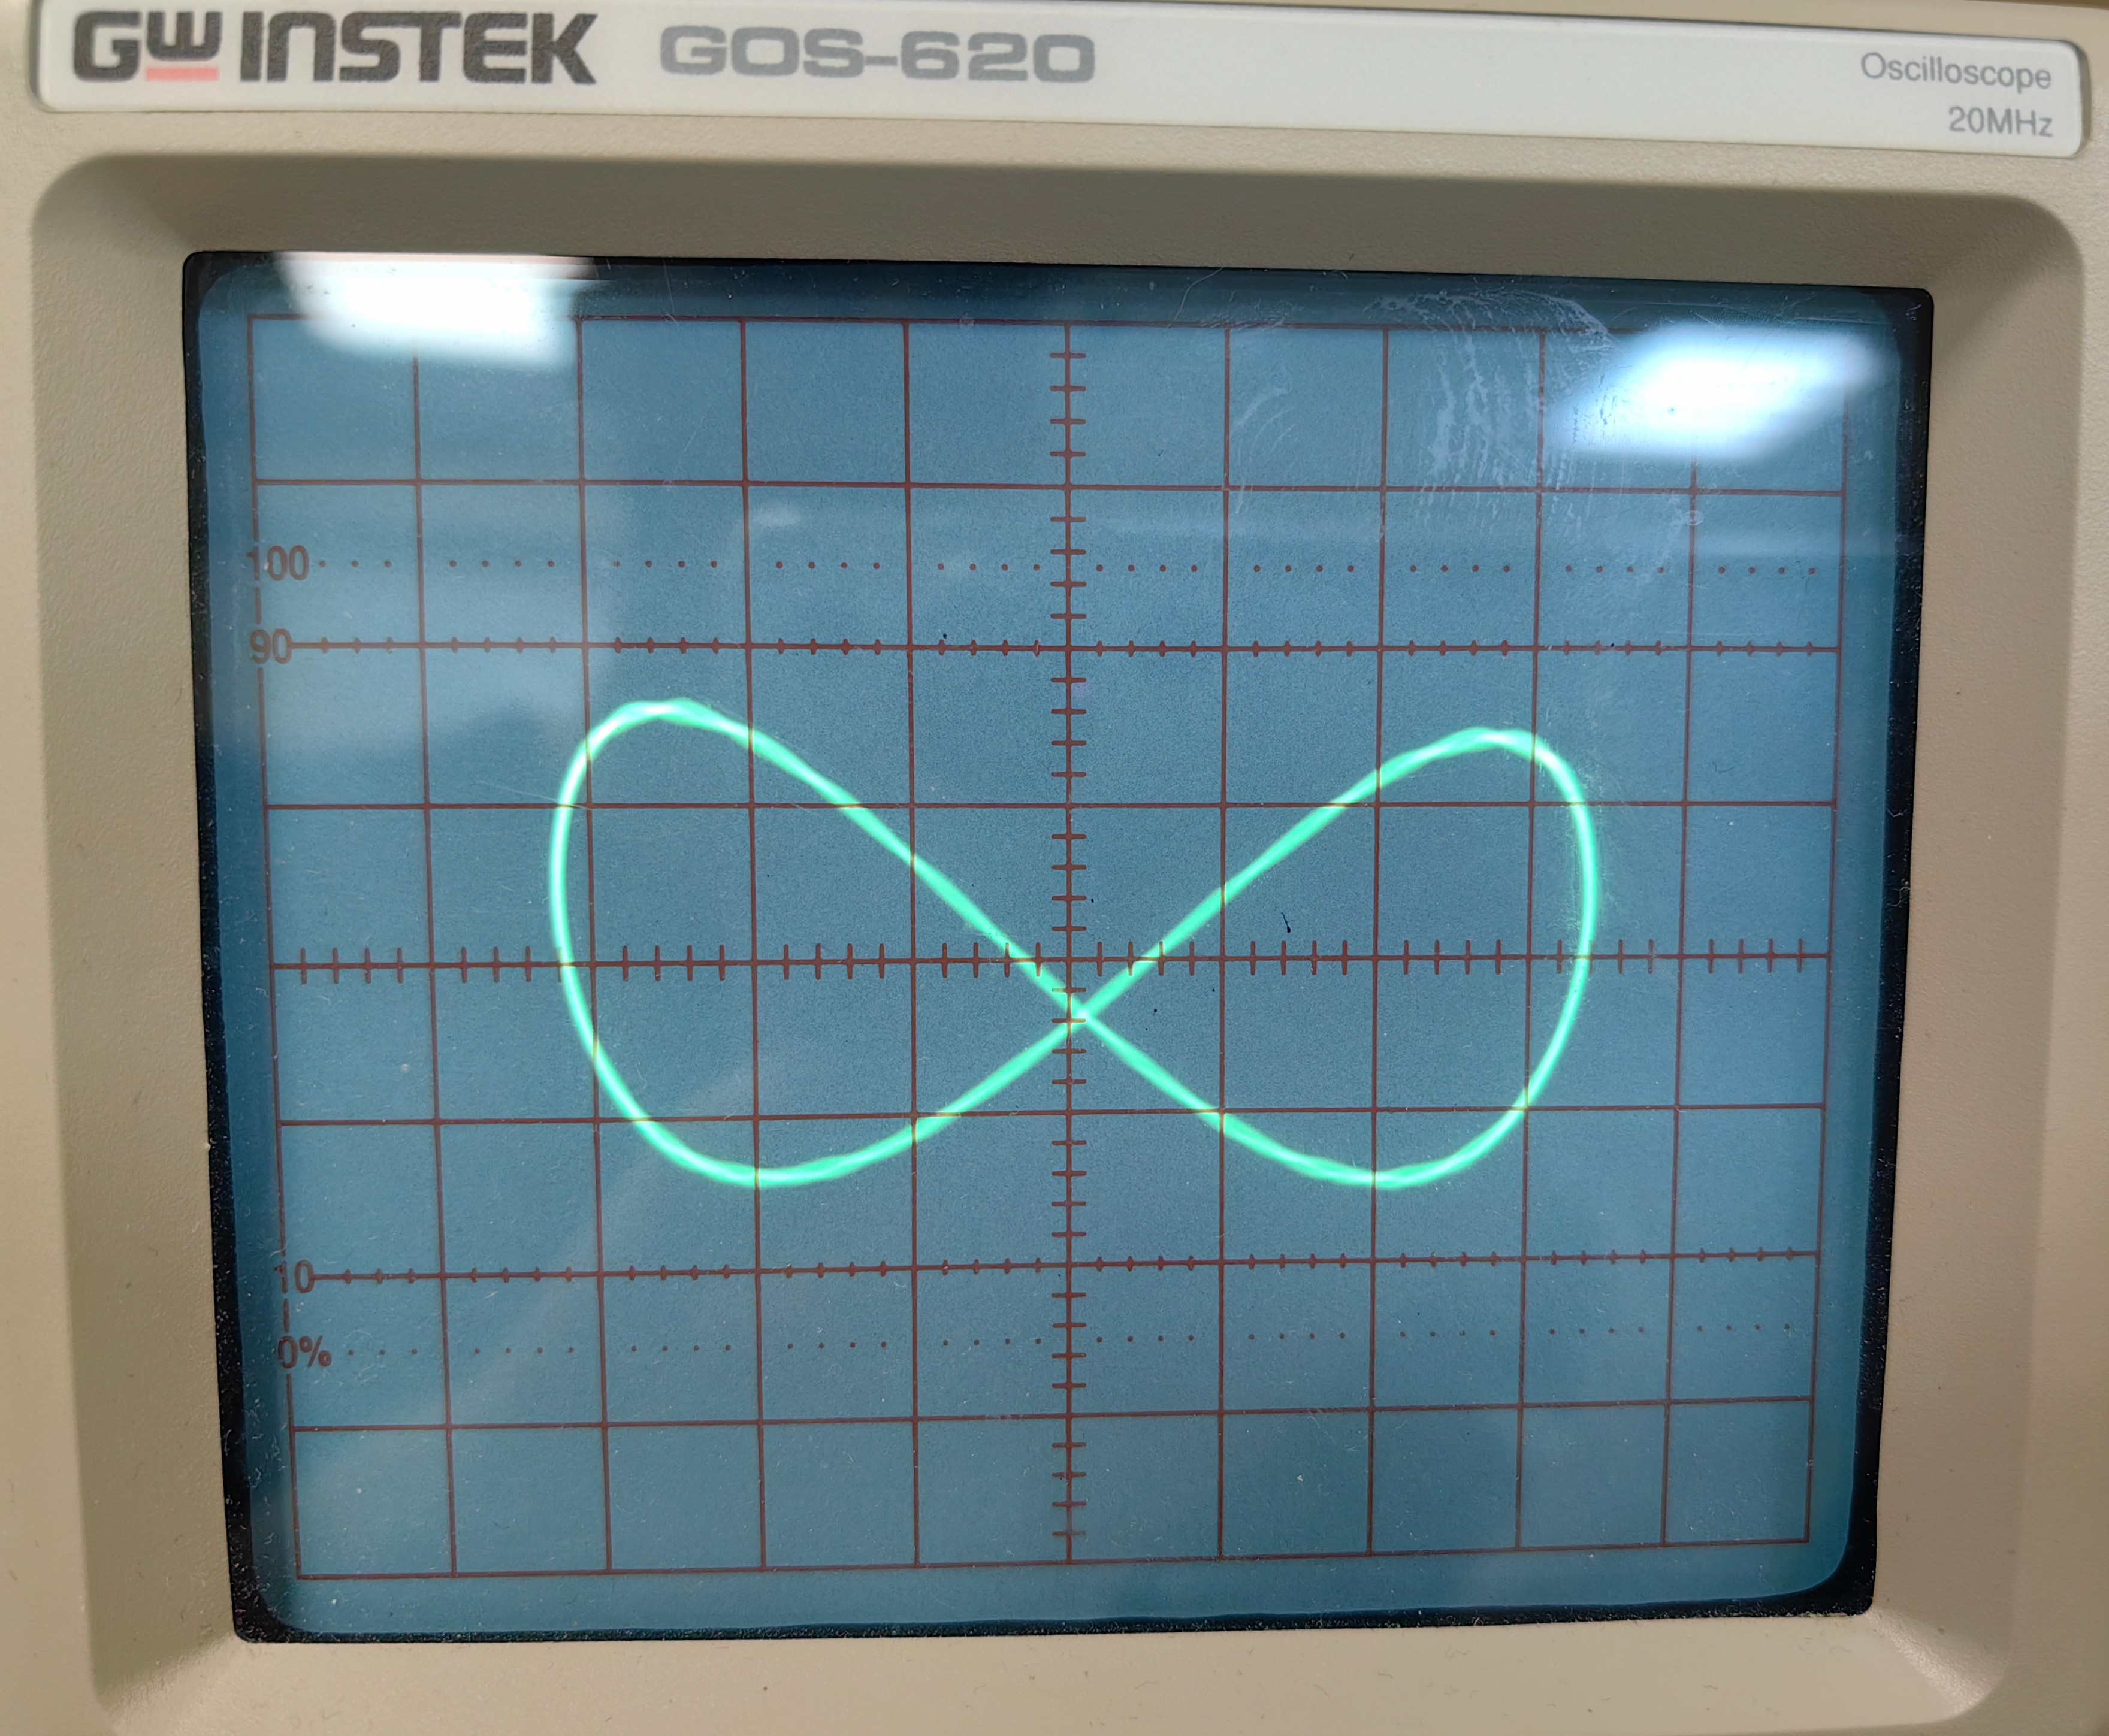
\includegraphics[scale=0.1]{data/butterfly}
  \caption{Бабочка на осциллографе.}
  \label{pic:6} \label{pic:butterfly}
\end{figure}

\item[12.] \label{Выполнение:12}
  Определим добротность стержня как колебательной системы, измерив амплитудно-частотную характеристику одного из стержней (лучше выбрать медный) вблизи первого резонанса. Найдите частоты $f_{11}$ и $f_{12}$, при которых амплитуда в $\sqrt{2}$ раз меньше максимальной, т.е. $A(f_1) = A(f_2) = A / \sqrt{2}$. Пусть $\D{f_1} = |f_{12} - f_{11}|$ Тогда добротность: $Q = \frac{f_1}{\D{f_1}}$. Уточните у преподавателя, как получить амплитуду на осциллографе.

\[ Q = 1449 \]

\item[13*.] \label{Выполнение:13}
  По указанию преподавателя повторите опыты 2-9 для стержней меньшей длины.

\begin{center}
  Не выполняли.
\end{center}

\subsection{Обработка результатов}

\item[14.] \label{Выполнение:14}
  Для каждого из исследованных стержней построим графики зависимости $f_n$ от n для каждого стержня, убедимся в их линейности и в том, что они проходят через начало координат (см. рис. \ref{pic:6}).
  
\begin{figure} [H] \center
  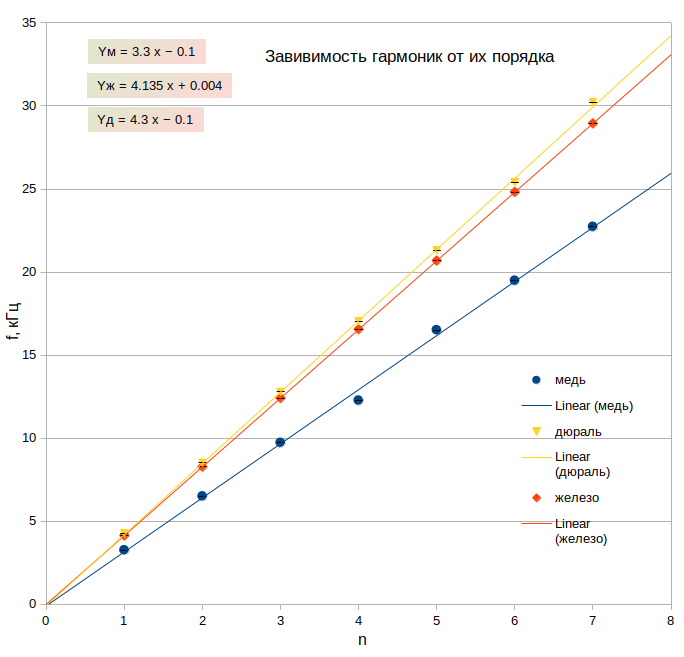
\includegraphics[scale=0.7]{data/f(n)}
  \caption{Графики зависимости $f_n$ от n для каждого стержня.}
  \label{pic:7}
\end{figure}

\item[15.] \label{Выполнение:15}
  Построим наилучшие прямые по экспериментальным точкам и определим скорости звука u.

Воспользуемся формулой \eqref{eq:15}.
\begin{equation}
  u = 2L \frac{f_n}{n}
  \label{eq:15(2)}
\end{equation}

Найдем скорость волн двумя способами: усреднив значения, полученные по формуле \ref{eq:15(2)} и по МНК.

\paragraph{Первый способ ($u = \avrg{u_n}$) (см. таблицу \ref{table:6})}: \\

$u_n = 2L \frac{f_n}{n}$ \\\\
$u = \avrg{u_n} = \avrg{2L \frac{f_n}{n}} = 2L \cdot \avrg{\frac{f_n}{n}}$ \\\\
$\sigma_u = \sqrt{(\sigma^{\text{случ}}_u)^2 + (\sigma^{\text{приб}}_u)^2} = \sqrt{STDEV(\{u_n\})^2 + \avrg{\sigma_{u_n}}^2}$

\begin{center}
  Таким образом:
\end{center}

% Таблица со скоростями, найденными по формуле 15(2)
\begin{table} [H] \center
\begin{tabular}{l|lll|lll|lll}
&Медь&&&Железо&&&Дюраль&&\\
\hline
&$u_n$, км/c&$\sigma_{u_n}$, км/c&$\eps_{u_n}$&$u_n$, км/c&$\sigma_{u_n}$, км/c&$\eps_{u_n}$&$u_n$, км/c&$\sigma_{u_n}$, км/c&$\eps_{u_n}$\\
\hline
1&3.91&0.01&0.2\%&4.96&0.01&0.2\%&5.11&0.01&0.2\%\\
2&3.90&0.01&0.2\%&4.97&0.01&0.2\%&5.11&0.01&0.2\%\\
3&3.89&0.01&0.2\%&4.96&0.01&0.2\%&5.11&0.01&0.2\%\\
4&3.68&0.01&0.2\%&4.97&0.01&0.2\%&5.11&0.01&0.2\%\\
5&3.96&0.01&0.2\%&4.96&0.01&0.2\%&5.11&0.01&0.2\%\\
6&3.90&0.01&0.2\%&4.96&0.01&0.2\%&5.08&0.01&0.2\%\\
7&3.90&0.01&0.2\%&4.96&0.01&0.2\%&5.18&0.01&0.2\%\\
\end{tabular}
\caption{Скорости в стержнях, найденные по формуле \eqref{eq:15(2)}}
\label{table:5}
\end{table}

% Таблица со средними значениями скоростей, найденных первым способом.
\begin{table} [H] \center
\begin{tabular}{l|lll}
&u, км/c&$\sigma_u$, км/c&$\eps_u$\\
\hline
Медь&3.88&0.09&2.3\%\\
Железо&4.96&0.01&0.2\%\\
Дюраль&5.12&0.03&0.6\%\\
\end{tabular}
\caption{Средние скорости }
\label{table:6}
\end{table}

\paragraph{Второй способ (МНК) (см. таблицу \ref{table:8})}: \\

  Пусть a - наклон прямой $f_n(n)$. \\\\
$f_n = a \cdot n = \frac{u}{2L} \cdot n \implies a = \frac{u}{2L}$ \\\\
$u = 2L \cdot a$ \\\\
$\sigma_u = u \cdot \sqrt{\eps_L^2 + \eps_a^2}$ \\\\
$\sigma_a$ находится по известной формуле из МНК:
\begin{equation}
  \sigma_a = \frac{1}{\sqrt{n}} \cdot 
  \sqrt{\frac{\avrg{y^2} - \avrg{y}^2}{\avrg{x^2} - \avrg{x}^2} - a^2}
  ,\quad (y = ax + b)
  \label{eq:slope error(1)}
\end{equation}
\begin{equation}
  \sigma_a = \frac{1}{\sqrt{n}} \cdot 
  \sqrt{\frac{\avrg{y^2}}{\avrg{x^2}} - a^2}
  ,\quad (y = ax)
  \label{eq:slope error(2)}
\end{equation}

Однако, эти формулы не учитывают приборные погрешности x и y.

\begin{center} Таким образом: (см. таблицу \ref{table:6} и \ref{table:7}) \end{center}

\begin{table} [H] \center
\begin{tabular}{l|lll|ll}
&a, кГц&$\sigma^1_a$, кГц&$\eps^1_a$&$\sigma^2_a$, кГц&$\eps^2_a$\\
\hline
Медь&3.24&0.13&4\%&0.07&2\%\\
Железо&4.14&0.10&2\%&0.09&2\%\\
Дюраль&4.25&0.23&5\%&0.17&4\%\\
\end{tabular}
\caption{Наклоны прямых.}
\label{table:7}
\end{table}

% Таблица со скоростями, найденными по МНК
\begin{table} [H] \center
\begin{tabular}{l|lll|ll}
&u, км/c&$\sigma^1_u$, км/c&$\eps^1_u$&$\sigma^2_u$, км/c&$\eps^2_u$\\
\hline
Медь&3.91&0.15&4\%&0.09&2\%\\
Железо&4.96&0.12&2\%&0.11&2\%\\
Дюраль&5.15&0.28&5\%&0.20&4\%\\
\end{tabular}
\caption{Скорости, найденные по МНК.}
\label{table:8}
\end{table}

% \paragraph{Третий способ ($u = \sqrt{\frac{E}{\rho}}$) (см. таблицу \ref{table:10})}Ж \\
% $\sigma_u = u \cdot \sqrt{\frac{\eps_E}{2}^2 + \frac{\eps_\rho}{2}^2}$ \\\\
% Считаем, что модули Юнга известны. \\
% \begin{table} [H] \center
% \begin{tabular}{l|lll}
% &E, $\frac{\kH}{\mm^2}$&$\sigma_E,\ \frac{\kH}{\mm^2}$&$\eps_E$\\
% \hline
% Медь&118&13&11\%\\
% Железо&195&5&3\%\\
% Дюраль&71&0&0\%\\
% \end{tabular}
% \caption{Модули юнга.}
% \label{table:9}
% \end{table}
% \begin{center} Таким образом: (см. таблицу \ref{table:9}) \end{center}
% \begin{table} [H] \center
% \begin{tabular}{l|lll}
% &u, км/c&$\sigma_u$, км/c&$\eps_u$\\
% \hline
% Медь&3.65&0.20&5\%\\
% Железо&5.00&0.09&2\%\\
% Дюраль&5.12&0.07&1\%\\
% \end{tabular}
% \caption{Скорости, найденные по по $u = \sqrt{\frac{E}{\rho}}$.}
% \label{table:10}
% \end{table}

\item[16.] \label{Выполнение:15}
  Определим модуль Юнга E по найденным значениям.

Воспользуемся формулой \eqref{eq:2}. \\\\
$u =  \sqrt{\frac{E}{\rho}}$ \\\\
$E = u^2 \rho, \quad \sigma_E = E \cdot \sqrt{(2\sigma_u)^2 + \sigma_\rho^2}$ \\\\

\begin{table} [H] \center
\begin{tabular}{l|lll}
&E, $\gPa$&$\sigma_E,\ \gPa$&$\eps_E$\\
\hline
Медь  &133&7&5.2\%\\
Железо&192&5&2.7\%\\
Дюраль&70 &2&2.9\%\\
\end{tabular}
\caption{Модули Юнга, полученные через скорости в таблице \ref{table:6}}
\label{table:9}
\end{table}

\begin{table} [H] \center
\begin{tabular}{l|lll}
&E, $\gPa$&$\sigma_E,\ \gPa$&$\eps_E$\\
\hline
Медь  &135&11& 8\%\\
Железо&192&10& 5\%\\
Дюраль& 71& 8&11\%\\
\end{tabular}
\caption{Модули Юнга, полученные через скорости в таблице \ref{table:8}}
\label{table:10}
\end{table}

\begin{table} [H] \center
\begin{tabular}{l|l}
&E, $\gPa$\\
\hline
Медь  &130\\
Железо&195\\
Дюраль& 71\\
\end{tabular}
\caption{Табличные Модули юнга.}
\label{table:11}
\end{table}

\item[17*.] Проделайте пункты 14-16 для маленьких стержней, если вы выполняли пункт \refb{Выполнение:13}.
\begin{center} Не выполняли. \end{center}

\end{enumerate}

\section{Вывод}
В данной работе мы экспериментально показали, что отношение резонантной частоты к номеру гармоники $f_n/n$ остается постоянным. Мы также вычислили значения скорости продольных волн в тонких стержнях, провели расчеты модуля Юнга для меди, стали и дюралюминия, которые совпали с табличными значениями в пределах погрешности.

\end{document}